
\documentclass[12pt]{article}

\usepackage[margin=1in]{geometry}
\usepackage{graphicx}

\title{Global Impact of Sea Level Rise Process Book}
\author{Brian Lavallee and Daniel Merrell}
\date{1 December 2019}

\begin{document}
	\maketitle

	\section{Overview and Motivation}
		Our goal was to create a visualization that had to do with climate change.
		We think that it is one of the most important issues the world faces today.
		Climate change has serious global impacts and we wanted to capture those impacts in our visualization.

		In particular, we wanted to create a visualization that showed the increasing effects of climate change over time.
		Many of the datasets we explored had metrics from weather stations around the world, but we struggled to think of ways in which we could use them to tell a story about people and individuals.
		We eventually found one that has the amount of impacted landmass by country for five different sea-level rise scenarios, from 1 meter to 5 meters.
		We decided to use this data set since sea-level rise is one of the impacts of climate change that unavoidably affects large coastal regions and populations.

	\section{Related Work}
		The paper\footnote{http://documents.worldbank.org/curated/en/156401468136816684/The-impact-of-sea-level-rise-on-developing-countries-a-comparative-analysis} that originally published the data is a study on the impact of sea level rise in developing countries.

	\section{Questions}
		We hoped to answer which countries are most affected by sea level rise.
		Through the course of the project, we began to thin more about how we could identify which populations are most affected by sea level rise.

	\section{Data}
		The central data source for our project is a study that details the amount of impacted area in coastal regions, mainly in undeveloped or developing countries.
		Furthermore, the dataset includes information on the population of the impacted regions and thus can provide insights into which countries are more at risk from the changing climate.
		There was relatively little data-wrangling for this dataset. The data was well-formed and complete.

		Although this is the information we wanted to explore the most, the tabular format is not as impactful as visually seeing how the coastlines of the world change as the sea-level rises.
		To add the map view, we incorporated three additional data sources.
		The primary data source is a digital elevation model produced by NASA called SRTM30.
		It gives average elevation in 1 arc-second squares, which are about 900 square meters (30x30) on the equator.
		Since the vast majority of the countries of interest all near or along the equator, this resolution is sufficient.
		NASA also provides two additional resolutions (SRTM3 and SRTM1) which measure elevation in 3mx3m squares and 1mx1m squares respectively.
		The extremely high resolution of these datasets is both unnecessary and intractable for visualization however since both are over 100GB in size.
		The model itself is simply a binary raster file split into 16 bit chunks.
		Each chunk gives the height of the corresponding cell, and the cells are laid out in row-major order in the raster.

		Although the digital elevation model (dem) could have been sufficient on its own, there was no way to distinguish between land at a negative elevation (potentially relative to some amount of sea level rise) and ocean.
		To rectify this so that we don’t visualize water incorrectly, we also use GTOPO30 to identify surface features.
		Although GTOPO30 does much more (in fact it also contains a dem, albeit less detailed and accurate), we only use it to identify ocean from land.
		Fortunately, the GTOPO30 dataset uses the same resolution and data format as SRTM30, and so compatibility was easy to manage and relatively built-in.

		Finally, we use the topographic maps from homework 4 to overlay countries on the map thereby enabling easier navigation within the map itself and adding stronger visual cues to match up impacted areas on the map with the data presented in the table.
		We used this data as is, although we did consider removing countries that do not appear in the sea-level rise dataset.

		After obtaining all of the data, there are a number of additional steps performed in the background of the visualization in order to convert the data into a map.
		The simplest in the country border data, where we simply convert the topojson to geojson, apply a projection (specifically Equirectangular to match the projection used by SRTM30), and then scale and translate to align it with the underlying map.

		A number of additional steps go into rendering the map itself.
		First, we perform a downselecting operation on the digital elevation model and surface features where the cells of a two dimensional grid are broken up into a smaller grid by considering the maximum value in nxn areas as a cell in the reduced grid.
		From here, the underlying technique is to pass the grid into the d3-contour library which produces a geojson object enclosing all of the cells above a given threshold.
		Although we could simply use the user-chosen sea level rise as the threshold on the dem, this approach also draws inland areas with negative elevation as underwater.
		To rectify this, we instead draw non-ocean surface features using GTOPO30.
		We create an auxiliary array where each cell is 0 if it is ocean and 1 otherwise which we can create directly from the GTOPO30 dataset.
		Using this array, we draw the lightblue contour to visualize the difference caused by the sea level rise.
		To determine what remains land, we efficiently simulate the spreading of the ocean using depth-first search from each ocean cell.
		If a land cell is below the sea-level rise and adjacent to an ocean cell, then it is remarked as an ocean cell.
		In this way, low lying areas of land which are surrounded by high lying areas are rendered as land, matching the natural phenomenon observed in the real world.
		The updated array is then passed into d3-contour with a threshold of 1 to visualize the remaining land as green.

	\section{Exploratory Data Analysis}
		Initially, we sought mainly to emulate the rendering below produced by NASA using the SRTM30 dataset.
		The image uses shading to depict elevation and thus gives a reasonably good intuition of which areas are low-lying and thus at risk.
		This gave us a good idea of what we should expect the visualization to look like and also informed our decision to use a slider to modulate the sea level rise.
		Without the slider, we found it difficult to tell apart the minor differences in elevation between nearby areas that determine underwater versus barely above.
		\newline

		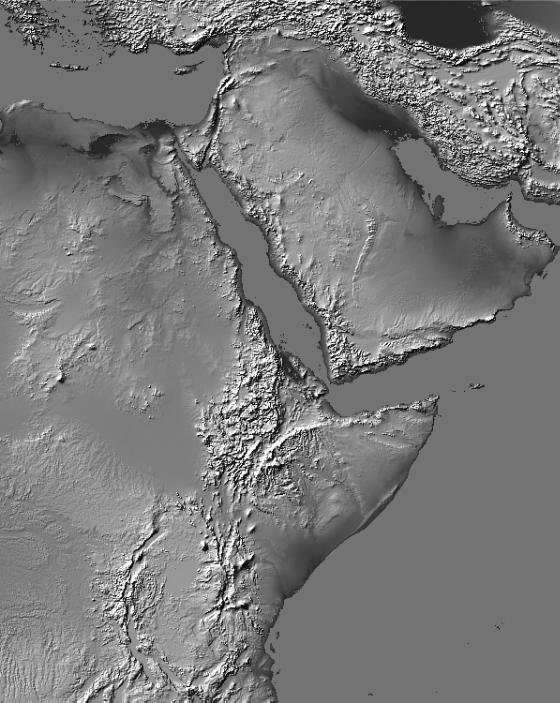
\includegraphics[scale=0.8]{images/data.png}

	\section{Design Evolution}
		The only major deviation from the proposal that we made was to visualize entire regions instead of single country in the map/country view.
		This drastically simplified the amount of data preprocessing that we needed to do while also giving more context around the area of interest.
		Originally, we also intended for the map to be completely non-interactive and only to update it based on input from the table.
		However, we found that it was very natural to want to see information about nearby countries based on the depicted impact, and searching the table for the correct country (assuming the user knows the country name) was tedious.
		Thus. we decided to add some minor navigational features to the map view itself.

		Within the table, instead of just displaying raw data, we wanted to include some type of meaningful visualization.
		We thought it would be interesting to include a bar in each row that showed the percent land mass affected per country, and the percent population affected.
		Though many people and large portions of land are affected in different sea-level rise scenarios, we realized that in most countries, the percentage is relatively small ($<5\%$).
		The bars ended up looking like slivers.
		After much thought, we decided to combine these data into a single column called ``Population density of Impacted Area.''
		We think this statistic is more interesting than the two independent numbers, and it was easily summarized by a bar.
		We also added a tooltip so you can see the exact number.

	\section{Implementation}
		\textbf{Info Box:}
		\newline

		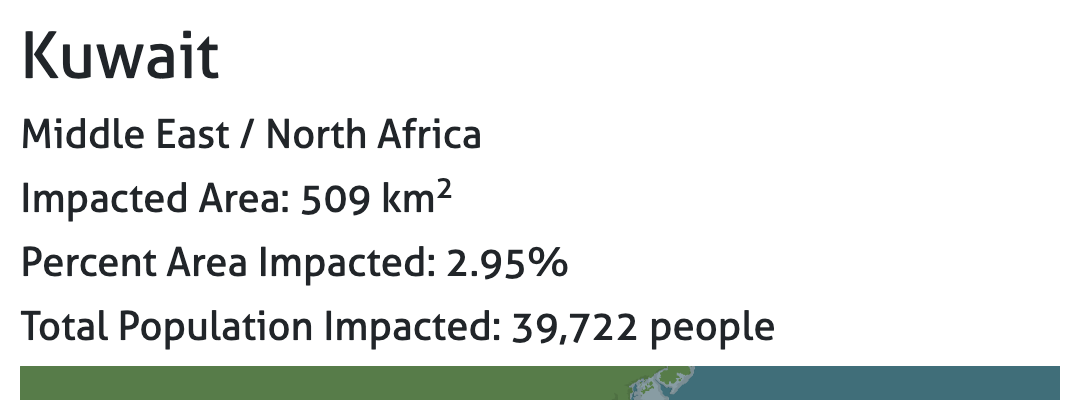
\includegraphics[scale=0.4]{images/infobox.png}
		\newline

		The info box shows information for the selected country.
		This information changes as the user slides the slider.
		\newline

		\textbf{Slider:}
		\newline

		
\includegraphics[scale=0.4]{images/slider.png}
		\newline

		Users can use the slider to see different sea level rise scenarios for the selected country.
		They can see different scenarios from 0-5 meters.
		Moving the slider updates the information in the info box and in the table.
		It also redraws the map.
		\newline\newline

		\textbf{Table:}
		\newline

		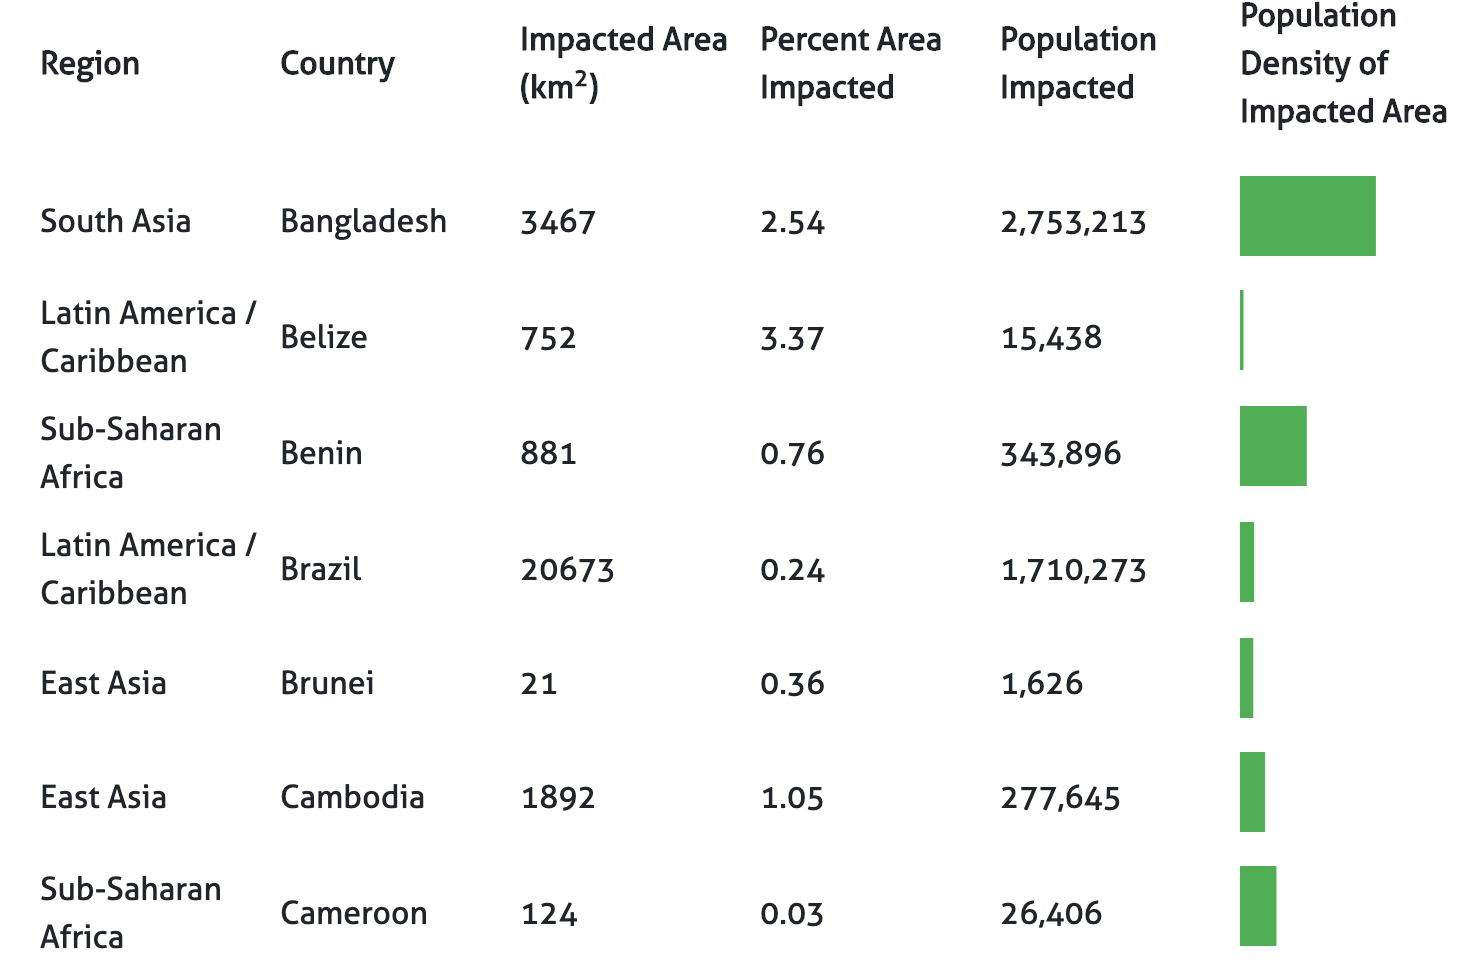
\includegraphics[scale=0.35]{images/table.png}
		\newline

		The table displays a list of countries, and the related info for the selected sea level rise scenario (set using the slider).
		The user can select any row in the table to see different sea level rise scenarios.
		The information in the table changes when the user changes the slider.
		The user is able to sort any of the columns by clicking the header.

		A tooltip is displayed when the user hovers over any bar.

		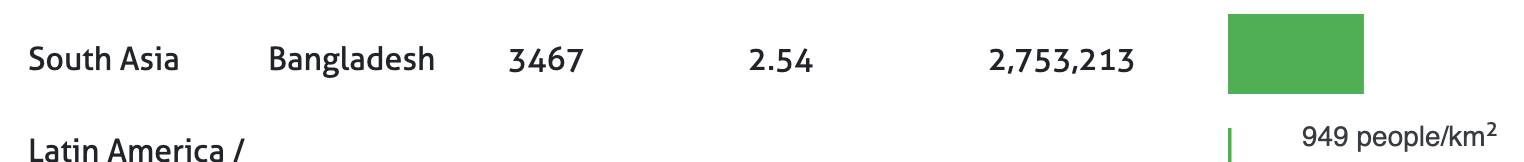
\includegraphics[scale=0.4]{images/tooltip.png}
		\newline

		\textbf{Map:}
		\newline

		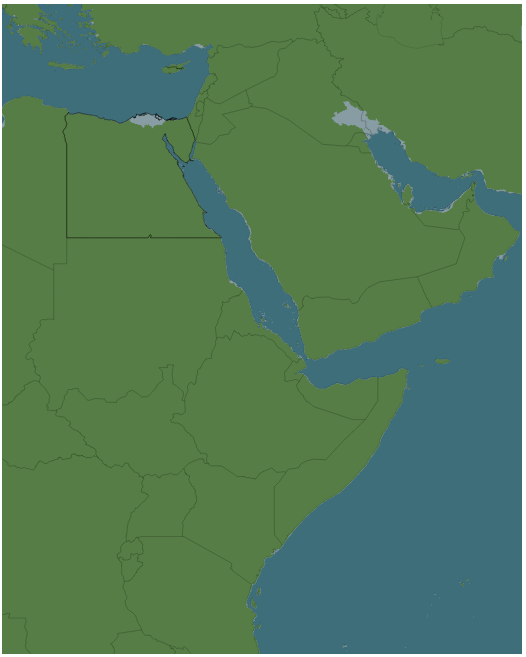
\includegraphics[scale=0.4]{images/map.png}
		\newline

		The map displays several key pieces of information.
		In lightblue, the coastline of every country is drawn when there is no sea level rise to that the change is easy to see.
		Above that in green, the land that remains after the sea level rise chosen on the slider is shown.
		Finally, the borders of each country are drawn in gray to provide context to the map.
		The outline of the selected country is darkened to direct attention.
		Finally, clicking on a country in the map (which is in the dataset) updates the info box and the highlight to include information about the clicked country.


	\section{Evaluation}
		We were able to answer both of our key questions simply by browsing in the visualization.
		Countries with large land impact include Bangladesh, China, and Egypt.
		The population density of impacted area metric also tells us that Egypt and Taiwan are at particularly high risk for human impact.
		Given these results, it would be interesting to explore the economic costs of replacing lost infrastructure including housing, industry, farmland, and other unrecoverable investments within each area.
		This question would require data and analysis far beyond the scope of this project, but is an interesting future direction.

		Although the map view does a good job visualizing the land that is impacted, without specific knowledge, it does a poor job communicating the population that is impacted.
		One simple addition would be to add markers for major cities in low lying areas.
		A more sophisticated approach that we considered would be to (optionally) overlay population density on the map.
		This would immediately direct users to areas with both lots of impacted area and population.
		Unfortunately, we were unable to find a dataset that would be easily compatible with our current data that was not intractably large for a browser based visualization.

		One major drawback of the map view is that it is completely static.
		Since the individual maps are relatively large, this doesn't affect most of the areas of interest.
		Nevertheless, several countries such as Brazil, Argentina, Thailand, and South Africa are split between multiple regions.
		In an updated version, we would add panning so that these countries can be brought into the center of the view.
		We note that this is a non-trivial task since it involves dynamically loading and aggregating several large datasets at once.
		In the same vein, another interesting feature to add would be zooming.
		Even using the SRTM30 resolution, we downselect the data before rendering to improve performance without meaningfully impacting the quality of the visualization.
		With a zoom feature, we could even consider adding the SRTM1 data and loading it instead when the extra resolution is needed.
		Combined with the population data, this would give users the opportunity to inspect specific cities or areas of interest.

\end{document}
